\documentclass[usenames,dvipsnames]{beamer}
\usepackage{../../shared/styles/custom}
\usepackage{../../shared/styles/conventions}
\usepackage{tikz}
\usetikzlibrary{arrows,shapes,positioning,shadows,trees,fit,calc}
\usepackage{pgfplots}
\pgfplotsset{compat=1.18}

\title{Seeing with Algorithms: Deep Dive into Object Detection}
\subtitle{From Classification to Localization and Detection Metrics}
\date{\today}
\author{Nipun Batra and teaching staff}
\institute{IIT Gandhinagar}

% Pop quiz counter is defined in theme-nipun.sty
\setcounter{popquiz}{0}

\begin{document}
	\maketitle
	
	% ===================================================================
	% Section 0: Setting the Stage
	% ===================================================================
	
	\begin{frame}{Learning Outcomes}
		\begin{itemize}
			\item Understand \textbf{classification}, \textbf{localization}, and \textbf{detection}
			\item Master \textbf{precision}, \textbf{recall}, \textbf{AP}, \textbf{mAP}, and \textbf{CA-mAP}
			\item Build strong intuition with toy examples and visual explanations
			\item Learn to evaluate object detectors thoroughly and effectively
		\end{itemize}
		
		\vspace{1em}
		\begin{center}
		\textit{"Detection is not just about finding objects, but finding them right."}
		\end{center}
	\end{frame}
	
	% Table of Contents
	\begin{frame}{Roadmap}
		\tableofcontents[hideallsubsections]
	\end{frame}
	
	% ===================================================================
	% Section 1: Classification vs Localization vs Detection
	% ===================================================================
	
	\section{Classification vs Localization vs Detection}
	
	\begin{frame}{Task Definitions}
		\begin{definitionbox}{Three Fundamental Computer Vision Tasks}
			\begin{itemize}
				\item \textbf{Classification}: What is present in the image?
				\item \textbf{Localization}: Where is the object in the image?
				\item \textbf{Detection} = Classification + Localization (for multiple objects)
			\end{itemize}
		\end{definitionbox}
		
		\vspace{1em}
		Each task builds upon the previous one, increasing in complexity and practical utility.
	\end{frame}
	
	\begin{frame}{Visual Examples}
		\begin{center}
		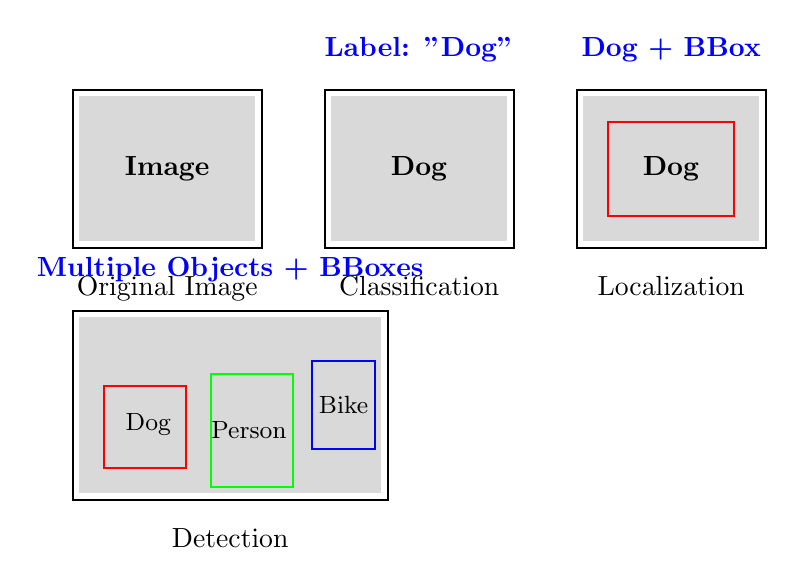
\begin{tikzpicture}[scale=0.8]
			% Base image representation
			\draw[thick] (0,0) rectangle (3,2.5);
			\fill[gray!30] (0.1,0.1) rectangle (2.9,2.4);
			\node at (1.5,1.25) {\textbf{Image}};
			\node[below] at (1.5,-0.3) {Original Image};
			
			% Classification
			\draw[thick] (4,0) rectangle (7,2.5);
			\fill[gray!30] (4.1,0.1) rectangle (6.9,2.4);
			\node at (5.5,1.25) {\textbf{Dog}};
			\node[below] at (5.5,-0.3) {Classification};
			\node[above, color=blue] at (5.5,2.8) {\textbf{Label: "Dog"}};
			
			% Localization
			\draw[thick] (8,0) rectangle (11,2.5);
			\fill[gray!30] (8.1,0.1) rectangle (10.9,2.4);
			\node at (9.5,1.25) {\textbf{Dog}};
			\draw[red, thick] (8.5,0.5) rectangle (10.5,2);
			\node[below] at (9.5,-0.3) {Localization};
			\node[above, color=blue] at (9.5,2.8) {\textbf{Dog + BBox}};
			
			% Detection
			\draw[thick] (0,-4) rectangle (5,-1);
			\fill[gray!30] (0.1,-3.9) rectangle (4.9,-1.1);
			\node at (1.2,-2.8) {\small Dog};
			\node at (2.8,-2.9) {\small Person};
			\node at (4.3,-2.5) {\small Bike};
			\draw[red, thick] (0.5,-3.5) rectangle (1.8,-2.2);
			\draw[green, thick] (2.2,-3.8) rectangle (3.5,-2);
			\draw[blue, thick] (3.8,-3.2) rectangle (4.8,-1.8);
			\node[below] at (2.5,-4.3) {Detection};
			\node[above, color=blue] at (2.5,-0.7) {\textbf{Multiple Objects + BBoxes}};
		\end{tikzpicture}
		\end{center}
	\end{frame}
	
	\begin{frame}{Output Formats}
		\begin{center}
		\begin{tabular}{|l|l|l|}
		\hline
		\textbf{Task} & \textbf{Output Format} & \textbf{Example} \\
		\hline
		Classification & \texttt{label} & \texttt{"dog"} \\
		\hline
		Localization & \texttt{label, bbox} & \texttt{"dog", (30,30,100,100)} \\
		\hline
		Detection & \texttt{[label, conf, bbox] × N} & \begin{tabular}[c]{@{}l@{}}
		\texttt{["dog", 0.95, (30,30,100,100)]} \\
		\texttt{["person", 0.87, (150,50,200,180)]} \\
		\texttt{["bike", 0.72, (80,120,140,200)]}
		\end{tabular} \\
		\hline
		\end{tabular}
		\end{center}
		
		\vspace{1em}
		\begin{keypointsbox}
		\textbf{Key Insight:} Detection outputs include confidence scores, enabling ranking and threshold-based filtering!
		\end{keypointsbox}
	\end{frame}
	
	% ===================================================================
	% Section 2: Bounding Boxes & Coordinates
	% ===================================================================
	
	\section{Bounding Boxes \& Coordinates}
	
	\begin{frame}{What is a Bounding Box?}
		\begin{definitionbox}{Bounding Box Formats}
			\begin{itemize}
				\item \textbf{Corner format}: $(x_{min}, y_{min}, x_{max}, y_{max})$
				\item \textbf{Center format}: $(x_{center}, y_{center}, width, height)$
			\end{itemize}
		\end{definitionbox}
		
		\begin{center}
		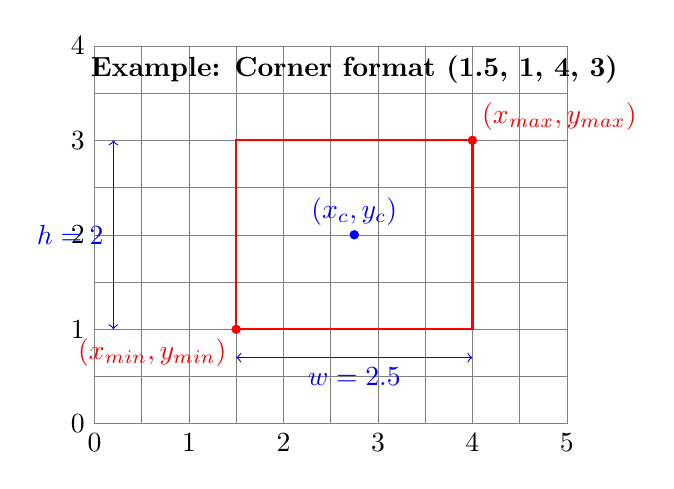
\begin{tikzpicture}[scale=1.2]
			% Grid
			\draw[help lines, step=0.5cm] (0,0) grid (5,4);
			\foreach \x in {0,1,2,3,4,5} \node[below] at (\x,0) {\x};
			\foreach \y in {0,1,2,3,4} \node[left] at (0,\y) {\y};
			
			% Bounding box
			\draw[red, thick] (1.5,1) rectangle (4,3);
			
			% Corner points
			\fill[red] (1.5,1) circle (0.05) node[below left] {$(x_{min}, y_{min})$};
			\fill[red] (4,3) circle (0.05) node[above right] {$(x_{max}, y_{max})$};
			
			% Center point
			\fill[blue] (2.75,2) circle (0.05) node[above] {$(x_c, y_c)$};
			
			% Dimensions
			\draw[<->, blue] (1.5,0.7) -- (4,0.7) node[midway, below] {$w = 2.5$};
			\draw[<->, blue] (0.2,1) -- (0.2,3) node[midway, left] {$h = 2$};
			
			\node[above] at (2.75,3.5) {\textbf{Example: Corner format (1.5, 1, 4, 3)}};
		\end{tikzpicture}
		\end{center}
	\end{frame}
	
	\begin{frame}{Ground Truth vs Predictions}
		\begin{center}
		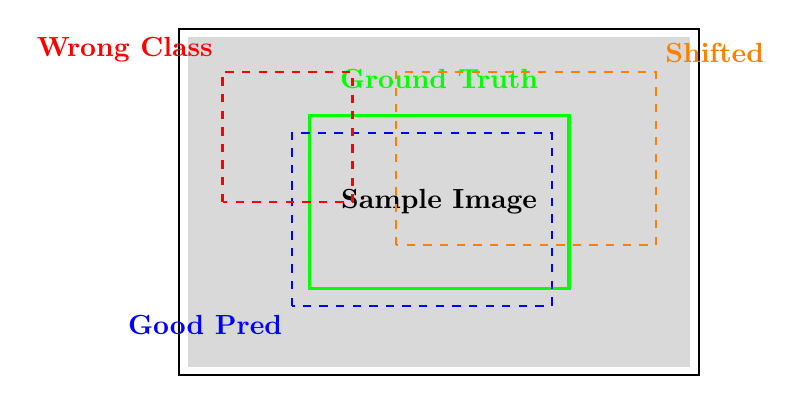
\begin{tikzpicture}[scale=1.1]
			% Image background
			\draw[thick] (0,0) rectangle (6,4);
			\fill[gray!30] (0.1,0.1) rectangle (5.9,3.9);
			\node at (3,2) {\textbf{Sample Image}};
			
			% Ground truth box
			\draw[green, very thick] (1.5,1) rectangle (4.5,3);
			\node[green, above] at (3,3.2) {\textbf{Ground Truth}};
			
			% Good prediction
			\draw[blue, thick, dashed] (1.3,0.8) rectangle (4.3,2.8);
			\node[blue, below left] at (1.3,0.8) {\textbf{Good Pred}};
			
			% Shifted prediction
			\draw[orange, thick, dashed] (2.5,1.5) rectangle (5.5,3.5);
			\node[orange, above right] at (5.5,3.5) {\textbf{Shifted}};
			
			% Wrong class prediction
			\draw[red, thick, dashed] (0.5,2) rectangle (2,3.5);
			\node[red, above left] at (0.5,3.5) {\textbf{Wrong Class}};
		\end{tikzpicture}
		\end{center}
		
		\begin{keypointsbox}
	\textbf{Matching Question:} How do we decide which predictions correspond to which ground truth objects?
		\end{keypointsbox}
	\end{frame}
	
	% ===================================================================
	% Section 3: IoU (Intersection over Union)
	% ===================================================================
	
	\section{IoU (Intersection over Union)}
	
	\begin{frame}{IoU Definition}
		\begin{definitionbox}{Intersection over Union (IoU)}
			$$\text{IoU} = \frac{\text{Area of Overlap}}{\text{Area of Union}} = \frac{|A \cap B|}{|A \cup B|}$$
		\end{definitionbox}
		
		\vspace{0.5em}
		\begin{center}
		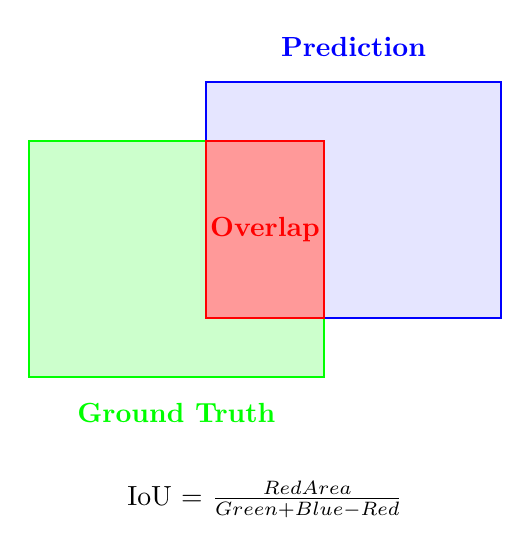
\begin{tikzpicture}[scale=1.5]
			% Ground truth box
			\draw[green, fill=green!20, thick] (0,0) rectangle (2.5,2);
			\node[green] at (1.25,-0.3) {\textbf{Ground Truth}};
			
			% Prediction box
			\draw[blue, fill=blue!20, thick, fill opacity=0.5] (1.5,0.5) rectangle (4,2.5);
			\node[blue] at (2.75,2.8) {\textbf{Prediction}};
			
			% Intersection
			\draw[red, fill=red!40, thick] (1.5,0.5) rectangle (2.5,2);
			\node[red] at (2,1.25) {\textbf{Overlap}};
			
			% Labels
			\node[below] at (2,-0.8) {IoU = $\frac{\text{Red Area}}{\text{Green + Blue - Red}}$};
		\end{tikzpicture}
		\end{center}
		
		\begin{itemize}
			\item \textbf{IoU = 1}: Perfect match
			\item \textbf{IoU = 0}: No overlap
			\item \textbf{IoU > 0.5}: Typically considered a "match"
		\end{itemize}
	\end{frame}
	
	\begin{frame}{IoU Calculation Example}
		\begin{examplebox}{Step-by-Step IoU Calculation}
			\textbf{Ground Truth}: $(30, 30, 100, 100)$ \\
			\textbf{Prediction}: $(50, 50, 120, 120)$
		\end{examplebox}
		
		\vspace{0.5em}
		\begin{columns}
		\column{0.5\textwidth}
		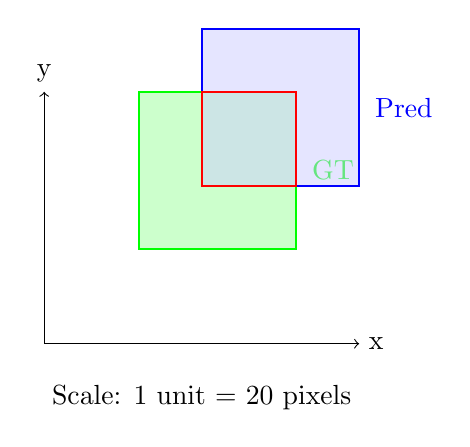
\begin{tikzpicture}[scale=0.8]
			% Coordinate system
			\draw[->] (0,0) -- (5,0) node[right] {x};
			\draw[->] (0,0) -- (0,4) node[above] {y};
			
			% Scale annotation
			\node[below] at (2.5,-0.5) {Scale: 1 unit = 20 pixels};
			
			% Ground truth
			\draw[green, fill=green!20, thick] (1.5,1.5) rectangle (4,4);
			\node[green, right] at (4.1,2.75) {GT};
			
			% Prediction
			\draw[blue, fill=blue!20, thick, fill opacity=0.5] (2.5,2.5) rectangle (5,5);
			\node[blue, right] at (5.1,3.75) {Pred};
			
			% Intersection
			\draw[red, thick] (2.5,2.5) rectangle (4,4);
		\end{tikzpicture}
		
		\column{0.5\textwidth}
		\textbf{Step 1: Find intersection} \\
		$x_{min} = \max(30, 50) = 50$ \\
		$y_{min} = \max(30, 50) = 50$ \\
		$x_{max} = \min(100, 120) = 100$ \\
		$y_{max} = \min(100, 120) = 100$ \\
		
		\textbf{Step 2: Calculate areas} \\
		Intersection: $50 \times 50 = 2500$ \\
		GT area: $70 \times 70 = 4900$ \\
		Pred area: $70 \times 70 = 4900$ \\
		Union: $4900 + 4900 - 2500 = 7300$ \\
		
		\textbf{Step 3: IoU} \\
		$\text{IoU} = \frac{2500}{7300} = 0.342$
		\end{columns}
	\end{frame}
	
	% ===================================================================
	% Section 4: Precision and Recall
	% ===================================================================
	
	\section{Precision and Recall}
	
	\begin{frame}{Definitions}
		\begin{definitionbox}{Core Metrics}
			$$\text{Precision} = \frac{TP}{TP + FP} \quad \text{Recall} = \frac{TP}{TP + FN}$$
		\end{definitionbox}
		
		\vspace{1em}
		\begin{itemize}
			\item \textbf{Precision}: What fraction of detections are correct? (Quality)
			\item \textbf{Recall}: What fraction of ground truth objects are detected? (Coverage)
			\item \textbf{TP}: True Positive (correct detection, IoU $\geq$ threshold)
			\item \textbf{FP}: False Positive (incorrect detection, IoU $<$ threshold or extra detection)
			\item \textbf{FN}: False Negative (missed ground truth object)
		\end{itemize}
		
		\begin{keypointsbox}
	\textbf{Intuition}
		High precision = few false alarms. High recall = few missed objects.
		\end{keypointsbox}
	\end{frame}
	
	\begin{frame}{Example: Counting TP, FP, FN}
		\begin{center}
		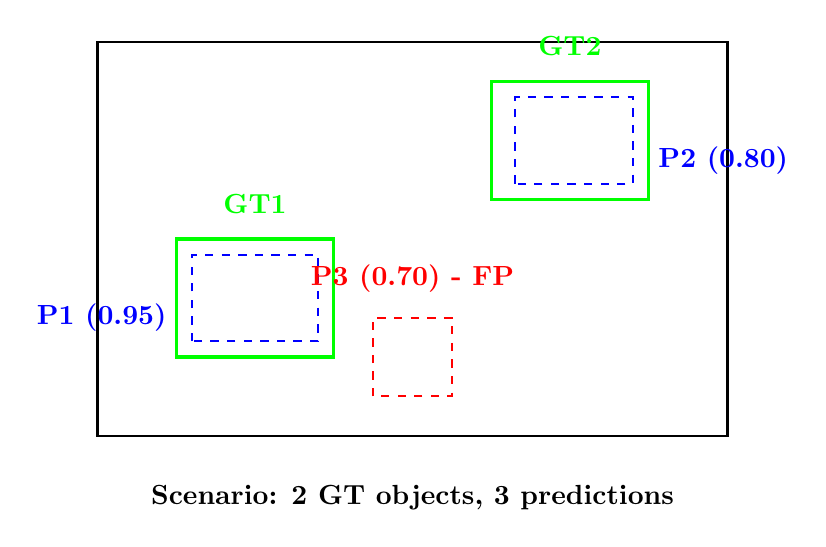
\begin{tikzpicture}[scale=1.0]
			\draw[thick] (0,0) rectangle (8,5);
			
			% Ground truth boxes (green)
			\draw[green, very thick] (1,1) rectangle (3,2.5);
			\node[green, above] at (2,2.7) {\textbf{GT1}};
			
			\draw[green, very thick] (5,3) rectangle (7,4.5);
			\node[green, above] at (6,4.7) {\textbf{GT2}};
			
			% Predictions
			% TP1: matches GT1 well
			\draw[blue, thick, dashed] (1.2,1.2) rectangle (2.8,2.3);
			\node[blue, left] at (1,1.5) {\textbf{P1 (0.95)}};
			
			% TP2: matches GT2 reasonably  
			\draw[blue, thick, dashed] (5.3,3.2) rectangle (6.8,4.3);
			\node[blue, right] at (7,3.5) {\textbf{P2 (0.80)}};
			
			% FP: no matching ground truth
			\draw[red, thick, dashed] (3.5,0.5) rectangle (4.5,1.5);
			\node[red, above] at (4,1.7) {\textbf{P3 (0.70) - FP}};
			
			\node[below] at (4,-0.5) {\textbf{Scenario: 2 GT objects, 3 predictions}};
		\end{tikzpicture}
		\end{center}
		
		\begin{columns}
		\column{0.5\textwidth}
		\textbf{Analysis} (IoU threshold = 0.5):
		\begin{itemize}
			\item P1 matches GT1: \textcolor{green}{\textbf{TP}}
			\item P2 matches GT2: \textcolor{green}{\textbf{TP}}  
			\item P3 no match: \textcolor{red}{\textbf{FP}}
			\item No missed GTs: \textbf{FN = 0}
		\end{itemize}
		
		\column{0.5\textwidth}
		\textbf{Metrics}:
		\begin{itemize}
			\item TP = 2, FP = 1, FN = 0
			\item Precision = $\frac{2}{2+1} = 0.667$
			\item Recall = $\frac{2}{2+0} = 1.000$
		\end{itemize}
		\end{columns}
	\end{frame}
	
	% ===================================================================
	% Section 5: Ranking and PR Curve
	% ===================================================================
	
	\section{Ranking and PR Curve}
	
	\begin{frame}{Ranked Predictions Table}
		\begin{examplebox}{Detection Results Sorted by Confidence}
			Given 5 predictions from our detector across the test set:
		\end{examplebox}
		
		\vspace{0.5em}
		\begin{center}
		\begin{tabular}{|c|c|c|c|}
		\hline
		\textbf{Confidence} & \textbf{Class} & \textbf{Box} & \textbf{TP/FP} \\
		\hline
		0.95 & Dog & (30,30,100,100) & \textcolor{green}{\textbf{TP}} \\
		\hline
		0.88 & Bike & (150,120,200,180) & \textcolor{red}{\textbf{FP}} \\
		\hline
		0.80 & Dog & (50,50,120,120) & \textcolor{green}{\textbf{TP}} \\
		\hline
		0.70 & Person & (200,50,280,150) & \textcolor{green}{\textbf{TP}} \\
		\hline
		0.40 & Cat & (100,100,150,150) & \textcolor{red}{\textbf{FP}} \\
		\hline
		\end{tabular}
		\end{center}
		
		\vspace{0.5em}
		\begin{keypointsbox}
		By varying the confidence threshold, we can trade off precision vs recall!
		\end{keypointsbox}
	\end{frame}
	
	\begin{frame}{Precision-Recall Table}
		\begin{center}
		\begin{tabular}{|c|c|c|c|c|c|}
		\hline
		\textbf{Threshold} & \textbf{Predictions} & \textbf{TP} & \textbf{FP} & \textbf{Precision} & \textbf{Recall} \\
		\hline
		0.95 & 1 & 1 & 0 & 1.000 & 0.333 \\
		\hline
		0.88 & 2 & 1 & 1 & 0.500 & 0.333 \\
		\hline
		0.80 & 3 & 2 & 1 & 0.667 & 0.667 \\
		\hline
		0.70 & 4 & 3 & 1 & 0.750 & 1.000 \\
		\hline
		0.40 & 5 & 3 & 2 & 0.600 & 1.000 \\
		\hline
		\end{tabular}
		\end{center}
		
		\vspace{0.5em}
		\textbf{Assumptions}: 3 ground truth objects total, IoU threshold = 0.5
		
		\vspace{0.5em}
		\begin{itemize}
			\item As threshold decreases → more predictions → recall increases
			\item But also more false positives → precision can decrease
		\end{itemize}
	\end{frame}
	
	\begin{frame}{Precision-Recall Curve}
		\begin{center}
		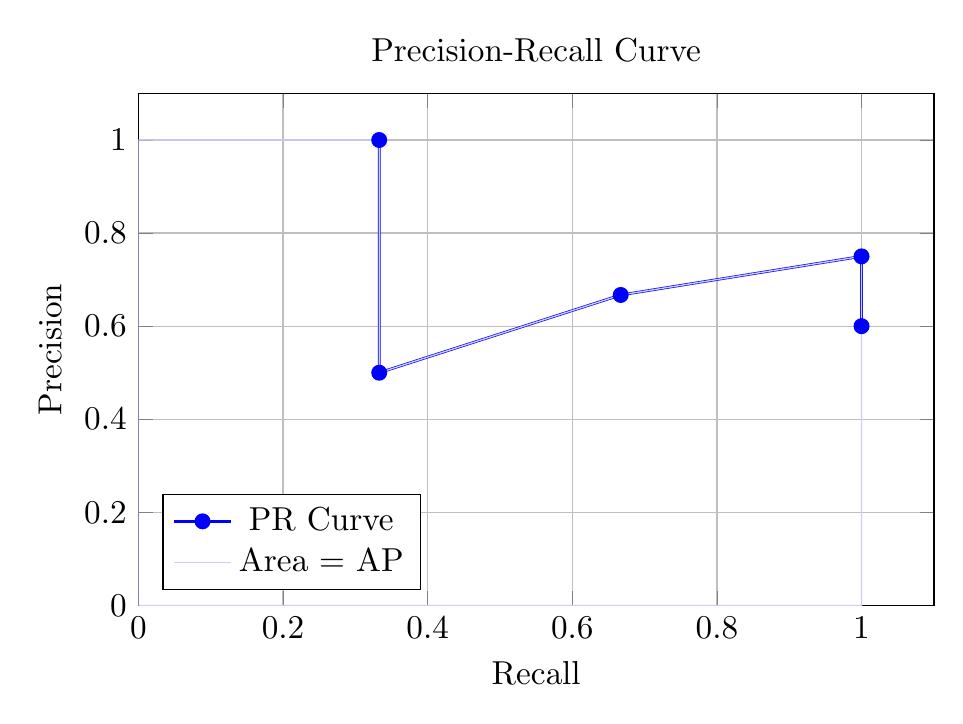
\begin{tikzpicture}[scale=1.2]
			\begin{axis}[
				width=10cm, height=7cm,
				xlabel={Recall},
				ylabel={Precision},
				xmin=0, xmax=1.1,
				ymin=0, ymax=1.1,
				grid=major,
				legend pos=south west,
				title={Precision-Recall Curve}
			]
			
			% PR curve points
			\addplot[mark=*, blue, thick] coordinates {
				(0.333, 1.000)
				(0.333, 0.500)
				(0.667, 0.667)
				(1.000, 0.750)
				(1.000, 0.600)
			};
			
			% Fill area under curve
			\addplot[blue!20, fill opacity=0.3] coordinates {
				(0, 1.000)
				(0.333, 1.000)
				(0.333, 0.500)
				(0.667, 0.667)
				(1.000, 0.750)
				(1.000, 0.600)
				(1.000, 0)
				(0, 0)
			} -- cycle;
			
			\legend{PR Curve, Area = AP}
			\end{axis}
		\end{tikzpicture}
		\end{center}
		
		\textbf{Average Precision (AP)} = Area under the PR curve = \textbf{0.72}
	\end{frame}
	
	% ===================================================================
	% Section 6: Average Precision (AP)
	% ===================================================================
	
	\section{Average Precision (AP)}
	
	\begin{frame}{AP = Area under PR Curve}
		\begin{definitionbox}{Average Precision Calculation}
			$$\text{AP} = \int_0^1 P(R) \, dR$$
			
			In practice: Numerical integration or 11-point interpolation
		\end{definitionbox}
		
		\vspace{1em}
		\begin{columns}
		\column{0.6\textwidth}
		\textbf{11-Point Interpolation}:
		\begin{itemize}
			\item Sample at recall levels: 0, 0.1, 0.2, ..., 1.0
			\item For each recall $r$, find max precision for recall $\geq r$
			\item Average the 11 precision values
		\end{itemize}
		
		\column{0.4\textwidth}
		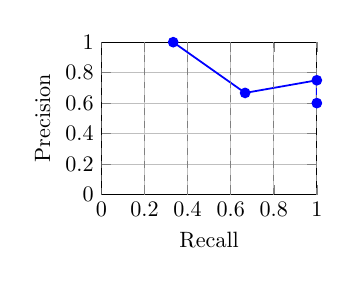
\begin{tikzpicture}[scale=0.8]
			\begin{axis}[
				width=5cm, height=4cm,
				xlabel={Recall},
				ylabel={Precision},
				xmin=0, xmax=1,
				ymin=0, ymax=1,
				grid=major
			]
			
			\addplot[mark=*, blue, thick] coordinates {
				(0.333, 1.000)
				(0.667, 0.667)
				(1.000, 0.750)
				(1.000, 0.600)
			};
			
			% Vertical lines for 11-point sampling
			\draw[gray, dashed] (axis cs:0,0) -- (axis cs:0,1);
			\draw[gray, dashed] (axis cs:0.2,0) -- (axis cs:0.2,1);
			\draw[gray, dashed] (axis cs:0.4,0) -- (axis cs:0.4,1);
			\draw[gray, dashed] (axis cs:0.6,0) -- (axis cs:0.6,1);
			\draw[gray, dashed] (axis cs:0.8,0) -- (axis cs:0.8,1);
			\draw[gray, dashed] (axis cs:1.0,0) -- (axis cs:1.0,1);
			\end{axis}
		\end{tikzpicture}
		\end{columns}
	\end{frame}
	
	\begin{frame}{Class-wise AP Example}
		\begin{center}
		\begin{tabular}{|l|c|c|}
		\hline
		\textbf{Class} & \textbf{AP@0.5} & \textbf{Visual} \\
		\hline
		Dog & 0.85 & \textcolor{green}{\textbf{Excellent}} \\
		\hline
		Person & 0.71 & \textcolor{orange}{\textbf{Good}} \\
		\hline
		Bicycle & 0.40 & \textcolor{red}{\textbf{Poor}} \\
		\hline
		\end{tabular}
		\end{center}
		
		\vspace{1em}
		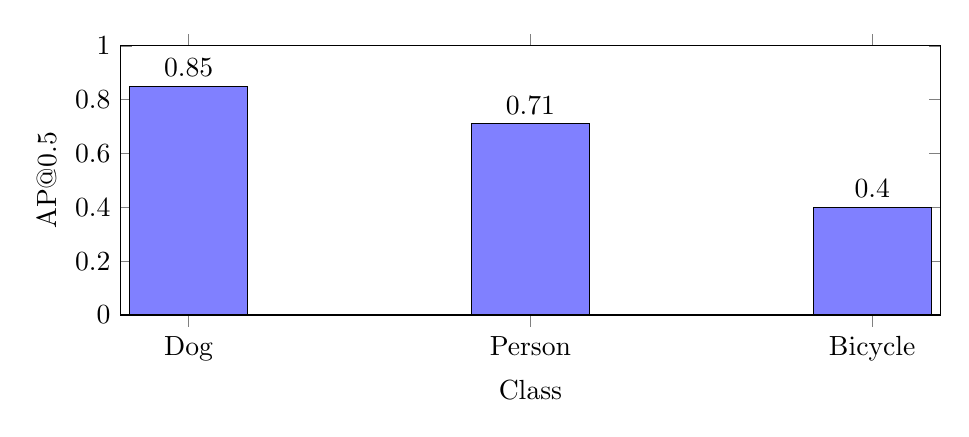
\begin{tikzpicture}[scale=1.0]
			\begin{axis}[
				width=12cm, height=5cm,
				ybar,
				bar width=1.5cm,
				xlabel={Class},
				ylabel={AP@0.5},
				ymin=0, ymax=1,
				symbolic x coords={Dog, Person, Bicycle},
				xtick=data,
				nodes near coords,
				nodes near coords align={vertical}
			]
			
			\addplot[fill=blue!50] coordinates {
				(Dog, 0.85)
				(Person, 0.71)
				(Bicycle, 0.40)
			};
			\end{axis}
		\end{tikzpicture}
		
		\textbf{Interpretation}: Dog detection works well, but bicycle detection needs improvement.
	\end{frame}
	
	% ===================================================================
	% Section 7: Mean AP and Class-Agnostic mAP
	% ===================================================================
	
	\section{Mean AP and Class-Agnostic mAP}
	
	\begin{frame}{Mean Average Precision (mAP)}
		\begin{definitionbox}{mAP Calculation}
			$$\text{mAP} = \frac{1}{C} \sum_{c=1}^{C} \text{AP}_c$$
			
			where $C$ is the number of classes
		\end{definitionbox}
		
		\vspace{1em}
		\begin{examplebox}{Our Example}
			$$\text{mAP} = \frac{\text{AP}_{dog} + \text{AP}_{person} + \text{AP}_{bicycle}}{3}$$
			$$= \frac{0.85 + 0.71 + 0.40}{3} = \textbf{0.653}$$
		\end{examplebox}
		
		\vspace{1em}
		\begin{keypointsbox}
	\textbf{Interpretation}
		mAP gives equal weight to all classes, regardless of their frequency in the dataset.
		\end{keypointsbox}
	\end{frame}
	
	\begin{frame}{Class-Agnostic mAP (CA-mAP)}
		\begin{definitionbox}{Class-Agnostic Evaluation}
			Ignore class labels when matching predictions to ground truth. \\
			Match based on IoU overlap alone.
		\end{definitionbox}
		
		\vspace{1em}
		\begin{columns}
		\column{0.5\textwidth}
		\textbf{Standard mAP}:
		\begin{itemize}
			\item Dog pred ↔ Dog GT: ✓
			\item Dog pred ↔ Person GT: ✗
		\end{itemize}
		
		\textbf{Class-Agnostic mAP}:
		\begin{itemize}
			\item Any pred ↔ Any GT (if IoU > threshold): ✓
			\item Useful for generic object detection
		\end{itemize}
		
		\column{0.5\textwidth}
		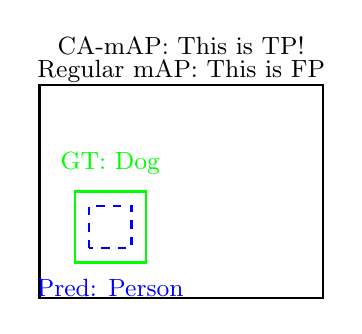
\begin{tikzpicture}[scale=0.9]
			\draw[thick] (0,0) rectangle (4,3);
			
			% GT boxes
			\draw[green, thick] (0.5,0.5) rectangle (1.5,1.5);
			\node[green, above] at (1,1.6) {\small GT: Dog};
			
			% Prediction box
			\draw[blue, thick, dashed] (0.7,0.7) rectangle (1.3,1.3);
			\node[blue, below] at (1,0.4) {\small Pred: Person};
			
			\node[above] at (2,3.3) {\small CA-mAP: This is TP!};
			\node[above] at (2,2.9) {\small Regular mAP: This is FP};
		\end{tikzpicture}
		\end{columns}
		
		\textbf{Use cases}: Weakly supervised learning, generic object detection, localization evaluation.
	\end{frame}

% ===================================================================
% Section 8: COCO-Style Evaluation  
% ===================================================================

\section{COCO-Style Evaluation}

\begin{frame}{Strict Evaluation: COCO Metrics}
	\begin{definitionbox}{COCO Evaluation Protocol}
		\begin{itemize}
			\item \textbf{AP@50}: IoU threshold = 0.5 (lenient)
			\item \textbf{AP@75}: IoU threshold = 0.75 (strict)  
			\item \textbf{AP@[.5:.95]}: Average over IoU thresholds 0.5, 0.55, 0.6, ..., 0.95
		\end{itemize}
	\end{definitionbox}
	
	\vspace{1em}
	\begin{center}
	\begin{tabular}{|l|c|c|}
	\hline
	\textbf{Metric} & \textbf{Value} & \textbf{Interpretation} \\
	\hline
	mAP@50 & 0.71 & Good localization (loose) \\
	\hline
	mAP@75 & 0.45 & Moderate precise localization \\
	\hline
	mAP@[.5:.95] & 0.42 & Overall localization quality \\
	\hline
	\end{tabular}
	\end{center}
	
	\begin{keypointsbox}
	\textbf{Key Insight}
	Higher IoU thresholds demand more precise localization!
	\end{keypointsbox}
\end{frame}

% ===================================================================
% Section 9: Interactive Quiz
% ===================================================================

\section{Interactive Quiz}

\begin{frame}{\stepcounter{popquiz}Pop Quiz \thepopquiz: Compute Precision \& Recall}
	\begin{popquizbox}{Pop Quiz \thepopquiz}
		Given the detection scenario below, compute precision and recall (IoU threshold = 0.5):
	\end{popquizbox}
	
	\vspace{0.5em}
	\begin{center}
	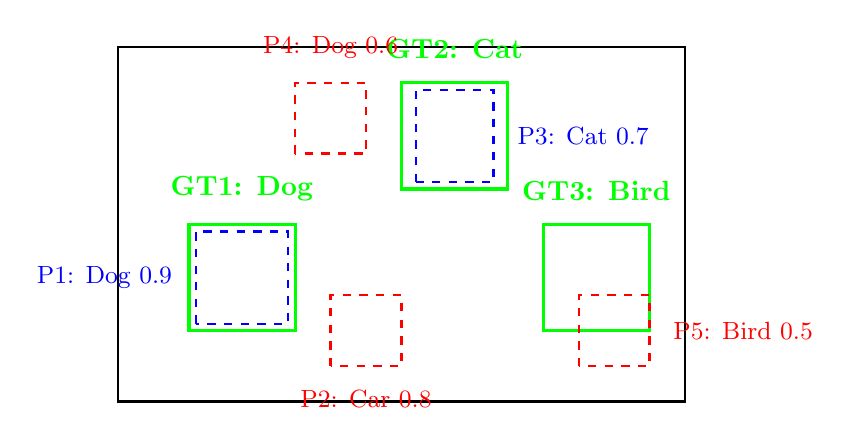
\begin{tikzpicture}[scale=0.9]
		\draw[thick] (0,0) rectangle (8,5);
		
		% 3 Ground truth boxes
		\draw[green, very thick] (1,1) rectangle (2.5,2.5);
		\node[green, above] at (1.75,2.7) {\textbf{GT1: Dog}};
		
		\draw[green, very thick] (4,3) rectangle (5.5,4.5);
		\node[green, above] at (4.75,4.7) {\textbf{GT2: Cat}};
		
		\draw[green, very thick] (6,1) rectangle (7.5,2.5);
		\node[green, above] at (6.75,2.7) {\textbf{GT3: Bird}};
		
		% 5 Predictions with confidence scores
		\draw[blue, thick, dashed] (1.1,1.1) rectangle (2.4,2.4);
		\node[blue, left] at (0.9,1.75) {\small P1: Dog 0.9};
		
		\draw[red, thick, dashed] (3,0.5) rectangle (4,1.5);
		\node[red, below] at (3.5,0.3) {\small P2: Car 0.8};
		
		\draw[blue, thick, dashed] (4.2,3.1) rectangle (5.3,4.4);
		\node[blue, right] at (5.5,3.75) {\small P3: Cat 0.7};
		
		\draw[red, thick, dashed] (2.5,3.5) rectangle (3.5,4.5);
		\node[red, above] at (3,4.7) {\small P4: Dog 0.6};
		
		\draw[red, thick, dashed] (6.5,0.5) rectangle (7.5,1.5);
		\node[red, right] at (7.7,1) {\small P5: Bird 0.5};
	\end{tikzpicture}
	\end{center}
	
	\textbf{Your task}: Count TP, FP, FN and compute Precision, Recall.
\end{frame}

\begin{frame}{Pop Quiz \thepopquiz: Answer}
	\begin{examplebox}{Solution}
		\textbf{Analysis} (with IoU > 0.5 matching):
		\begin{itemize}
			\item P1 (Dog 0.9) matches GT1 (Dog): \textcolor{green}{\textbf{TP}}
			\item P2 (Car 0.8) no GT match: \textcolor{red}{\textbf{FP}}
			\item P3 (Cat 0.7) matches GT2 (Cat): \textcolor{green}{\textbf{TP}}  
			\item P4 (Dog 0.6) no GT match: \textcolor{red}{\textbf{FP}}
			\item P5 (Bird 0.5) poor overlap with GT3: \textcolor{red}{\textbf{FP}}
			\item GT3 (Bird) unmatched: \textcolor{orange}{\textbf{FN}}
		\end{itemize}
	\end{examplebox}
	
	\vspace{0.5em}
	\textbf{Final counts}: TP = 2, FP = 3, FN = 1
	
	$$\text{Precision} = \frac{2}{2+3} = 0.40 \quad \text{Recall} = \frac{2}{2+1} = 0.67$$
\end{frame}

% ===================================================================
% Section 10: Summary and Wrap-up
% ===================================================================

\section{Summary \& Takeaways}

\begin{frame}{Summary Table}
	\begin{center}
	\begin{tabular}{|l|l|l|}
	\hline
	\textbf{Concept} & \textbf{Meaning} & \textbf{Key Insight} \\
	\hline
	IoU & Box overlap quality & Matching criterion (usually > 0.5) \\
	\hline
	Precision & Detection quality & $\frac{TP}{TP + FP}$ (fewer false alarms) \\
	\hline
	Recall & Detection coverage & $\frac{TP}{TP + FN}$ (fewer missed objects) \\
	\hline
	AP & Area under PR curve & Single-class performance metric \\
	\hline
	mAP & Average AP over classes & Multi-class detector performance \\
	\hline
	CA-mAP & Class-agnostic mAP & Localization-only evaluation \\
	\hline
	COCO & Multi-IoU evaluation & AP@[.5:.95] for precise localization \\
	\hline
	\end{tabular}
	\end{center}
	
	\vspace{1em}
	\begin{keypointsbox}
	\textbf{Golden Rule}
	\textbf{"Detection is not just about finding objects, but finding them right."}
	\end{keypointsbox}
\end{frame}

\begin{frame}{What We've Learned}
	\begin{itemize}
		\item \textbf{Task hierarchy}: Classification → Localization → Detection
		\item \textbf{Evaluation pipeline}: IoU matching → TP/FP counting → PR curves → AP/mAP
		\item \textbf{Trade-offs}: Precision vs Recall, lenient vs strict IoU thresholds
		\item \textbf{Practical metrics}: COCO-style evaluation for real-world deployment
	\end{itemize}
	
	\vspace{1em}
	\begin{center}
	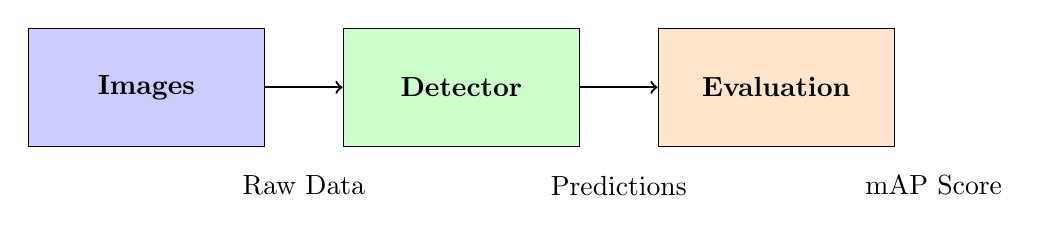
\begin{tikzpicture}[scale=1.0]
		\node[rectangle, draw, fill=blue!20, minimum width=3cm, minimum height=1.5cm] (box1) at (0,0) {\textbf{Images}};
		\node[rectangle, draw, fill=green!20, minimum width=3cm, minimum height=1.5cm] (box2) at (4,0) {\textbf{Detector}};
		\node[rectangle, draw, fill=orange!20, minimum width=3cm, minimum height=1.5cm] (box3) at (8,0) {\textbf{Evaluation}};
		
		\draw[->, thick] (box1) -- (box2);
		\draw[->, thick] (box2) -- (box3);
		
		\node[below] at (2,-1) {Raw Data};
		\node[below] at (6,-1) {Predictions};
		\node[below] at (10,-1) {mAP Score};
	\end{tikzpicture}
	\end{center}
	
	\textbf{Next steps}: Explore modern architectures (YOLO, R-CNN, Transformers) and their mAP performance!
\end{frame}

\end{document}
